\documentclass[12pt]{article}
\linespread{1.25}
\usepackage{times}

\usepackage{pgfplots}
\pgfplotsset{compat = newest}
\usetikzlibrary{positioning, arrows.meta}
\usepgfplotslibrary{fillbetween}
\usepackage{amsmath}

\begin{document}

\begin{center}
\hspace*{-3cm}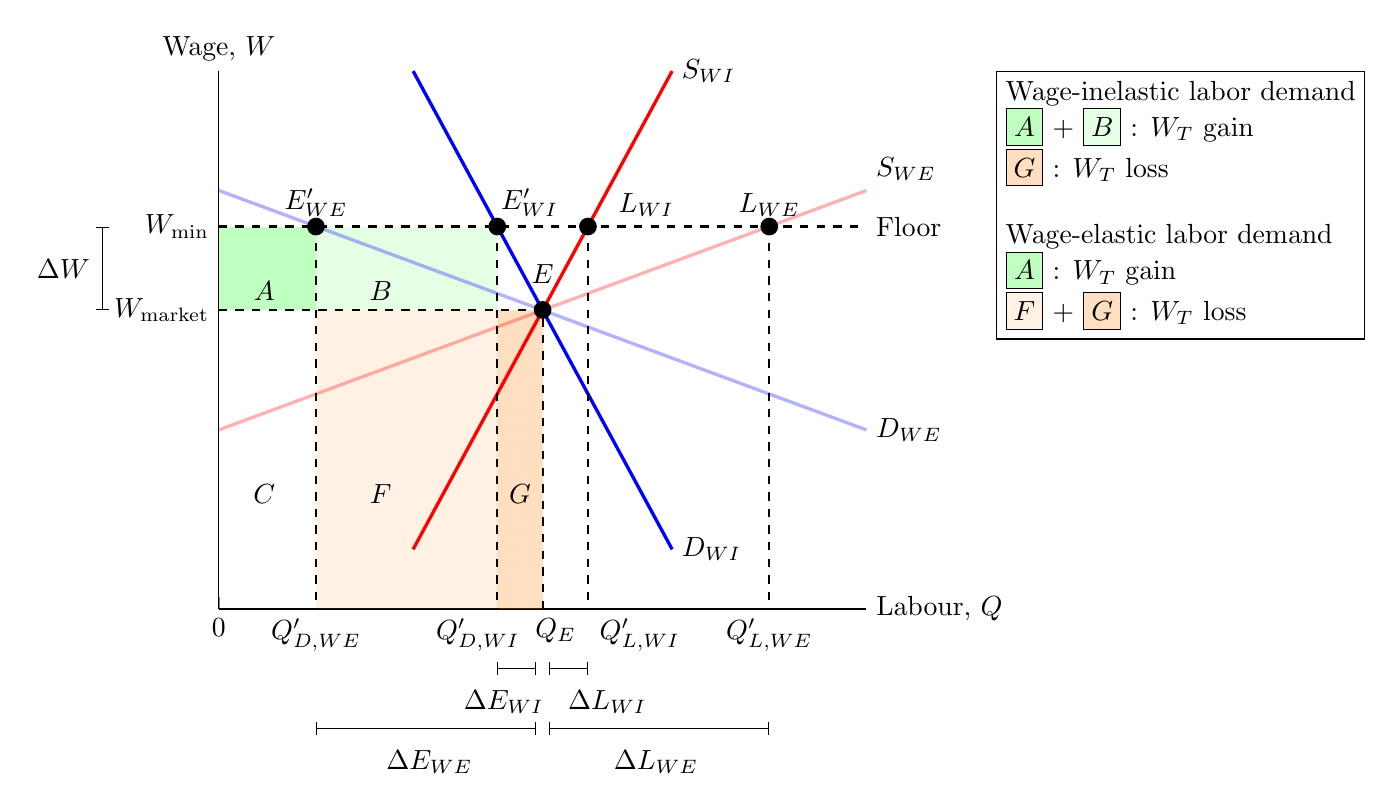
\begin{tikzpicture}
\begin{axis}[
scale = 1.2,
xmin = 0, xmax = 10,
ymin = 0, ymax = 10,
axis lines* = left,
xtick = {0}, ytick = \empty,
clip = false,
]
% Colouring areas
\fill[green, opacity = 0.25] (0, 7.11) -- (1.5, 7.11) -- (1.5, 5.56) -- (0, 5.56);
\fill[green, opacity = 0.1] (1.5, 7.11) -- (1.5, 5.56) -- (4.3, 5.56) -- (4.3, 7.11);
\fill[orange, opacity = 0.25] (4.3, 0) -- (5, 0) -- (5, 5.56) -- (4.3, 5.56);
\fill[orange, opacity = 0.1] (4.3, 0) -- (4.3, 5.56) -- (1.5, 5.56) -- (1.5, 0);

% Supply and Demand Curves
\node [above] at (current axis.above origin) {Wage, $W$};
\node [right] at (current axis.right of origin) {Labour, $Q$};
\addplot[color = blue, very thick, opacity = 0.3] coordinates {(0, 7.78) (10, 3.33)};
\addplot[color = blue, very thick] coordinates {(3, 10) (7, 1.11)};
\addplot[color = red, very thick, opacity = 0.3] coordinates{(0, 3.33) (10, 7.78)};
\addplot[color = red, very thick] coordinates{(3, 1.11) (7, 10)};

% Wage Floor
\addplot[color = black, dashed, thick] coordinates {(0, 7.11) (10, 7.11)};

% Quantity and Price Lines
\addplot[color = black, dashed, thick] coordinates {(0, 5.56) (5, 5.56) (5, 0)};
\addplot[color = black, dashed, thick] coordinates {(1.5, 7.11) (1.5, 0)};
\addplot[color = black, dashed, thick] coordinates {(4.3, 7.11) (4.3, 0)};
\addplot[color = black, dashed, thick] coordinates {(5.7, 7.11) (5.7, 0)};
\addplot[color = black, dashed, thick] coordinates {(8.5, 7.11) (8.5, 0)};

% Labels: E, L
\addplot[color = black, mark = *, only marks, mark size = 3pt] coordinates {(1.5, 7.11) (4.3, 7.11) (5, 5.56) (5.7, 7.11) (8.5, 7.11)};
\node [above=6pt] at (5, 5.56) {$E$};
\node [above] at (1.5, 7.11) {$E^{\prime}_{WE}$};
\node [above] at (4.8, 7.11) {$E^{\prime}_{WI}$};
\node [above] at (6.6, 7.11) {$L_{WI}$};
\node [above] at (8.5,7.11) {$L_{WE}$};

% Labels: S, D
\node [right] at (10, 3.33) {$D_{WE}$};
\node [above right] at (10, 7.78) {$S_{WE}$};
\node [right] at (7, 1.11) {$D_{WI}$};
\node [right] at (7, 10) {$S_{WI}$};
\node [left] at (0, 5.56) {$W_{\text{market}}$};
\node [left] at (0, 7.11) {$W_{\text{min}}$};
\node [below] at (1.5, 0) {$Q^{\prime}_{D, WE}$};
\node [below] at (4, 0) {$Q^{\prime}_{D, WI}$};
\node [below] at (5.2, 0) {$Q_E$};
\node [below] at (6.5, 0) {$Q^{\prime}_{L, WI}$};
\node [below] at (8.5, 0) {$Q^{\prime}_{L, WE}$};
\node [right] at (10, 7.11) {Floor};
\node [above] at (0.7, 5.56) {$A$};
\node [above] at (0.7, 1.78) {$C$};
\node [above] at (2.5, 5.56) {$B$};
\node [above] at (2.5, 1.78) {$F$};
\node [above] at (4.65, 1.78) {$G$};

% Dimension indicators
\draw[|-|] (4.3, -1.11) to (4.9, -1.11);
\node [below] at (4.4, -1.33) {$\Delta E_{WI}$};
\draw[|-|] (5.1, -1.11) to (5.7, -1.11);
\node [below] at (6, -1.33) {$\Delta L_{WI}$};
\draw[|-|] (1.5, -2.22) to (4.9, -2.22);
\node [below] at (3.25, -2.44) {$\Delta E_{WE}$};
\draw[|-|] (5.1, -2.22) to (8.5, -2.22);
\node [below] at (6.75, -2.44) {$\Delta L_{WE}$};
\draw[|-|] (-1.8, 5.56) to (-1.8, 7.11);
\node [below] at (-2.4, 6.67) {$\Delta W$};

% Legend
\node[below right, draw, align = left] at (12, 10) {
Wage-inelastic labor demand \\
\fcolorbox{black}{green!25}{\makebox[\fontcharht\font`X]{$A$}} + \fcolorbox{black}{green!10}{\makebox[\fontcharht\font`X]{$B$}} : $W_T$ gain \\
\fcolorbox{black}{orange!25}{\makebox[\fontcharht\font`X]{$G$}} : $W_T$ loss \\ \\
Wage-elastic labor demand \\
\fcolorbox{black}{green!25}{\makebox[\fontcharht\font`X]{$A$}} : $W_T$ gain \\
\fcolorbox{black}{orange!10}{\makebox[\fontcharht\font`X]{$F$}} + \fcolorbox{black}{orange!25}{\makebox[\fontcharht\font`X]{$G$}} : $W_T$ loss 
};
\end{axis}
\end{tikzpicture}\hspace*{-3cm}
\end{center}
\textbf{Figure 0-1:} Wage elasticities and total income.

\end{document}
